\documentclass[a4paper,12pt]{article}

%Мои доработки
\usepackage[margin=10pt,font=small,labelfont=bf,
labelsep=period]{caption} % позволяет центровать подписи и издеваться над caption
%\usepackage{float} %здесь здесь, только здесь
\usepackage{floatrow} %нельзя одновременно включать floatrow и float
\usepackage{graphicx} %два пакета для размещения картинки и таблицы в ряд
%%% Работа с русским языком
\usepackage{enumitem} % развлекаться со списками
% объявляем новую команду для переноса строки внутри ячейки таблицы
\newcommand{\specialcell}[2][c]{%
	\begin{tabular}[#1]{@{}c@{}}#2\end{tabular}}
%	\renewcommand{\arraystretch}{1.8} %% increase table row spacing
%	\renewcommand{\tabcolsep}{1cm}   %% increase table column spacing


\usepackage{cmap}					% поиск в PDF
\usepackage{mathtext} 				% русские буквы в формулах
\usepackage[T2A]{fontenc}			% кодировка
\usepackage[utf8]{inputenc}			% кодировка исходного текста
\usepackage[english,russian]{babel}	% локализация и переносы

%%% Дополнительная работа с математикой
\usepackage{amsmath,amsfonts,amssymb,amsthm,mathtools} % AMS
\usepackage{icomma} % "Умная" запятая: $0,2$ --- число, $0, 2$ --- перечисление

%% Номера формул
%\mathtoolsset{showonlyrefs=true} % Показывать номера только у тех формул, на которые есть \eqref{} в тексте.
%\usepackage{leqno} % Нумерация формул слева

%% Свои команды
\DeclareMathOperator{\sgn}{\mathop{sgn}}

%% Перенос знаков в формулах (по Львовскому)
\newcommand*{\hm}[1]{#1\nobreak\discretionary{}
	{\hbox{$\mathsurround=0pt #1$}}{}}

%%% Работа с картинками
\usepackage{graphicx}  % Для вставки рисунков
\graphicspath{{images/}{images2/}}  % папки с картинками
\setlength\fboxsep{3pt} % Отступ рамки \fbox{} от рисунка
\setlength\fboxrule{1pt} % Толщина линий рамки \fbox{}
\usepackage{wrapfig} % Обтекание рисунков текстом

%%% Работа с таблицами
\usepackage{array,tabularx,tabulary,booktabs} % Дополнительная работа с таблицами
\usepackage{longtable}  % Длинные таблицы
\usepackage{multirow} % Слияние строк в таблице

%%% Теоремы
\theoremstyle{plain} % Это стиль по умолчанию, его можно не переопределять.
\newtheorem{theorem}{Теорема}[section]
\newtheorem{proposition}[theorem]{Утверждение}

\theoremstyle{definition} % "Определение"
\newtheorem{corollary}{Следствие}[theorem]
\newtheorem{problem}{Задача}[section]

\theoremstyle{remark} % "Примечание"
\newtheorem*{nonum}{Решение}

%%% Программирование
\usepackage{etoolbox} % логические операторы

%%% Страница
\usepackage{extsizes} % Возможность сделать 14-й шрифт
\usepackage{geometry} % Простой способ задавать поля
\geometry{top=25mm}
\geometry{bottom=35mm}
\geometry{left=35mm}
\geometry{right=20mm}
%

\usepackage{fancyhdr} % Колонтитулы
\pagestyle{fancy}
\renewcommand{\sectionmark}[1]{\markboth{#1}{}}
%\renewcommand{\headrulewidth}{0mm}  % Толщина линейки, отчеркивающей верхний колонтитул
%\lfoot{Нижний левый}
%\rfoot{Нижний правый}
%\rhead{}
%\chead{Верхний в центре}
\lhead{\thepage}
\cfoot{} % По умолчанию здесь номер страницы

\usepackage{setspace} % Интерлиньяж
%\onehalfspacing % Интерлиньяж 1.5
%\doublespacing % Интерлиньяж 2
%\singlespacing % Интерлиньяж 1

\usepackage{lastpage} % Узнать, сколько всего страниц в документе.

\usepackage{soul} % Модификаторы начертания

\usepackage{indentfirst} % Красная строка

\usepackage{soulutf8} % Модификаторы начертания

%\usepackage{hyperref}
%\usepackage[usenames,dvipsnames,svgnames,table,rgb]{xcolor}
%\hypersetup{				% Гиперссылки
%	unicode=true,           % русские буквы в раздела PDF
%	pdftitle={Заголовок},   % Заголовок
%	pdfsubject={Тема},      % Тема
%	pdfcreator={Создатель}, % Создатель
%	pdfproducer={Производитель}, % Производитель
%	pdfkeywords={keyword1} {key2} {key3}, % Ключевые слова
%	colorlinks=true,       	% false: ссылки в рамках; true: цветные ссылки
%	linkcolor=red,          % внутренние ссылки
%	citecolor=green,        % на библиографию
%	filecolor=magenta,      % на файлы
%	urlcolor=cyan           % на URL
%}

%\renewcommand{\familydefault}{\sfdefault} % Начертание шрифта


\usepackage{multicol} % Несколько колонок

\author{\LaTeX{} в Вышке}
\title{3.2 Оформление документа в целом}
\date{\today}

\begin{document} % конец преамбулы, начало документа
	\thispagestyle{empty}
	\begin{center}
		\textit{Федеральное государственное автономное образовательное\\ учреждение высшего образования }
		\vspace{0.5ex}
		
		\textbf{«Московский физико-технический институт\\ (национальный исследовательский университет)»}
	\end{center}
	\vspace{10ex}
	%\begin{flushright}
	%	\noindent
	%	\textit{Фамилия Имя Отчество}
	%	\\
	%	\textit{студент факультета экономики \\(группа 211И)}
	%\end{flushright}
	\begin{center}
		\vspace{13ex}
		\so{\textbf{Лабораторная работа №2.1.6}}
		\vspace{1ex}
		
		по курсу общей физики
		
		
		на тему:
		
		\textbf{\textit{<<Эффект Джоуля-Томсона>>}}
		\vspace{30ex}
		\begin{flushright}
			\noindent
			\textit{Работу выполнил:}
			\\
			\textit{Баринов Леонид \\(группа Б02-827)}
		\end{flushright}
		\vfill
		Долгопрудный \\2019
	\end{center}
	\newpage
	\setcounter{page}{1}
	\fancyhead[R]{\nouppercase{\leftmark}}
	\section{Аннотация}
	В работе будет определено изменение температуры углекислого газа при протекании через малопроницаемую перегородку при разных начальных значениях давления и температуры
	
	Будет произведено вычисление по результатам опытов коэффициентов Ван-дер-Ваальса <<$a$>> и <<$b$>>.
	\section {Теоретические сведения}
	\subsection{Эффект Джоуля-Томсона}
	Эффектом Джоуля-Томсона называется изменение температуры газа, медленно протекающего из области высокого в область низкого давления в условиях хорошей тепловой изоляции. В разреженных газах, которые приближаются по своим свойствам к идеальному газу, при таком течении температура газа не меняется. Эффект Джоуля-Томсона демонстрирует отличие исследуемого газа от идеального.
	\subsection{Определение величины эффекта Джоуля-Томсона}
	В работе исследуется изменение температуры углекислого газа при медленном его течении по трубке с пористой перегородкой (Рис. 1). Трубка 1 хорошо теплоизолирована. Газ из области повышенного давления $P_1$ проходит через множество узких и длинных каналов пористой перегородки 2 в область с атмосферным давлением $Р_2$. Перепад давления $\Delta P = P_1 -P_2$ из-за большого сопротивления каналов может быть заметным даже при малой скорости течения газа в трубке. Величина эффекта Джоуля-Томсона определяется по разности температуры газа до и после перегородки.
	
	Рассмотрим стационарный поток газа между произвольными сечениями $I$ и $II$ трубки (до перегородки и после нее). Пусть, для определенности, через трубку прошел $1 \text{моль}$ углекислого газа; $\mu$ — его молярная масса. Молярные объемы газа, его давления и отнесенные к молю внутренние энергии газа в сечениях  $I$ и $II$ обозначим соответственно $V_1$, $P_1$, $U_1$ и $V_2$, $P_2$, $U_2$. Для того чтобы ввести в трубку объем $V_1$ над газом нужно совершить работу $A_1 = P_1 V_1$. Проходя через сечение $II$, газ сам совершает работу $A_2 = P_2 V_2$. Так как через боковые стенки не происходит ни обмена теплом, ни передачи механической энергии, то
	\begin{equation}
	A_1 - A_2 = \left(U_2 + \frac{\mu \upsilon_2^2}{2}\right) - \left(U_1 + \frac{\mu \upsilon_1^2}{2}\right)
	\end{equation}
	В уравнении (1) учтено изменение как внутренней (первые члены в скобках), так и кинетической (вторые члены в скобках) энергии газа. Подставляя в (1) написанные выражения для $A_1$ и $A_2$ и перегруппировывая члены, найдем
	\begin{equation}
	H_1 - H_2 = (U_1 + P_1V_1)-(U_2+P_2V_2) = \frac{1}{2} \mu (\upsilon_2^2-\upsilon_1^2)
	\end{equation}
	\begin{figure}[H]
		\begin{center}
			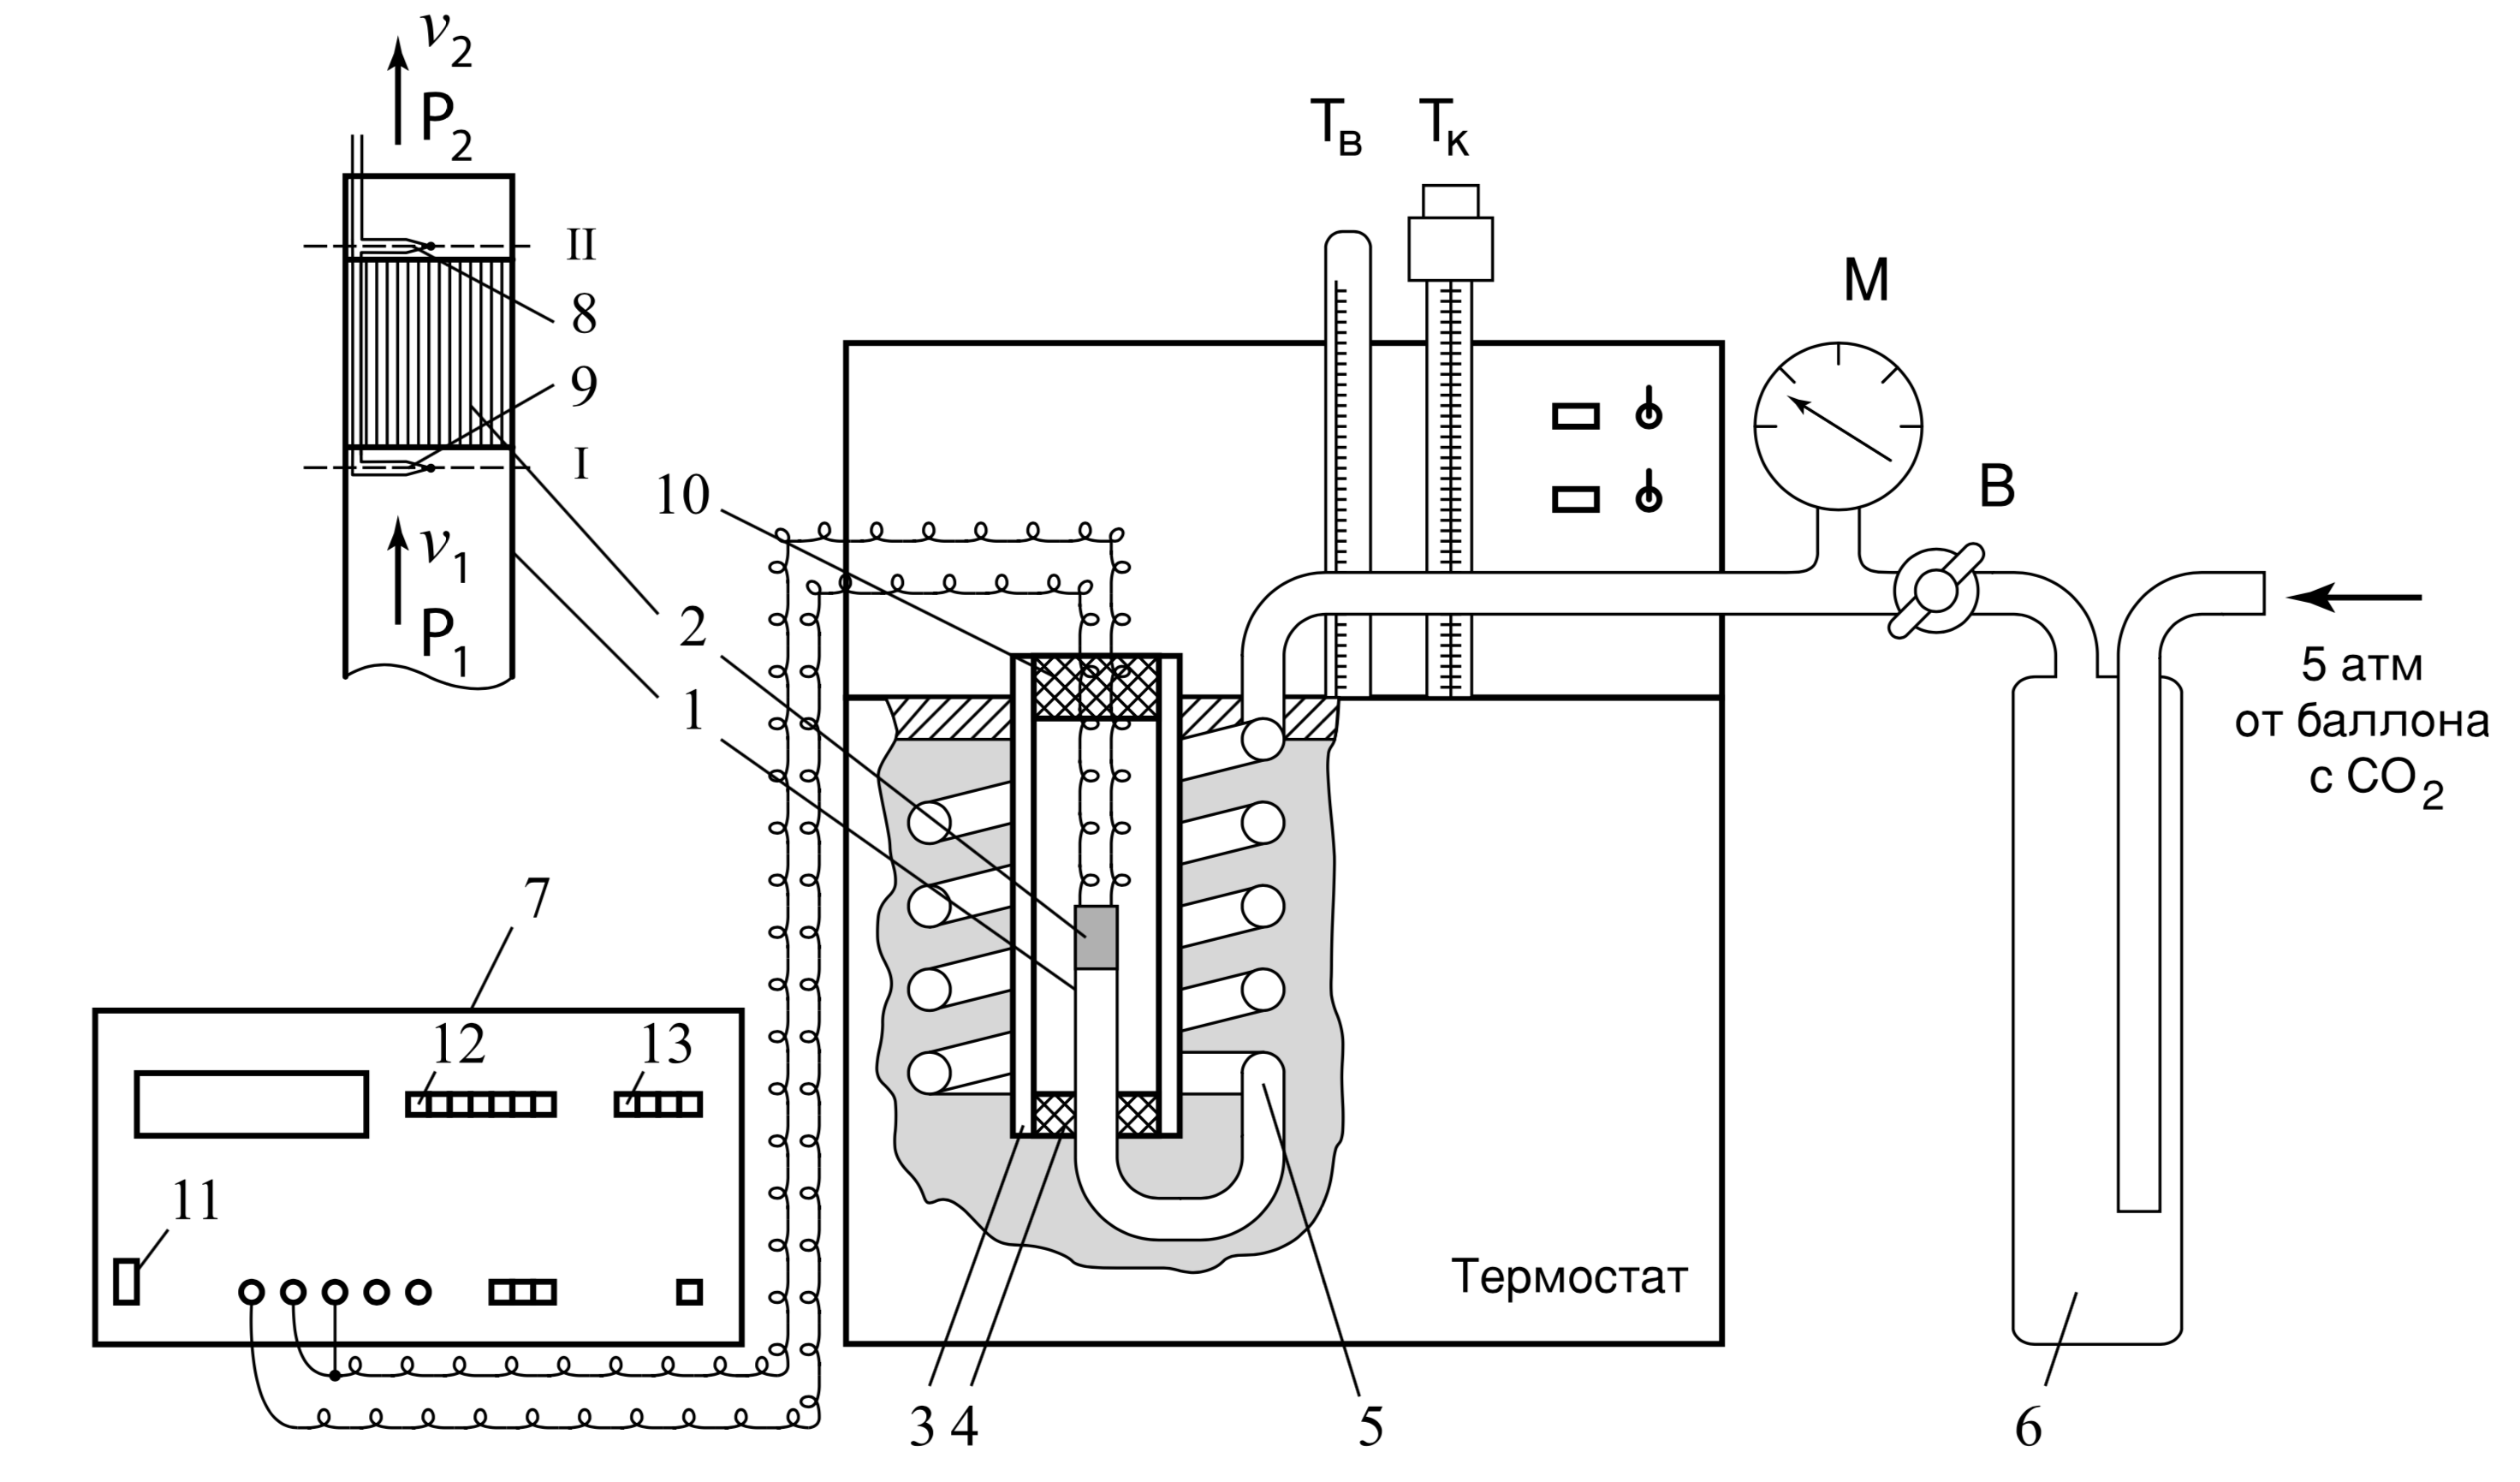
\includegraphics[width=\linewidth]{1}
			\captionsetup{justification=centering}
			\caption{Схема установки для изучения эффекта Джоуля-Томсона}
		\end{center}
	\end{figure}
Сделаем несколько замечаний. Прежде всего отметим, что в процессе Джоуля-Томсона газ испытывает в пористой перегородке существенное трение, приводящее к ее нагреву. Потери энергии на нагрев трубки в начале процесса могут быть очень существенными и сильно искажают ход явления. После того как температура трубки установится и газ станет уносить с собой все выделенное им в пробке тепло, формула (1) становится точной, если, конечно, теплоизоляция трубки достаточно хороша и не происходит утечек тепла наружу через ее стенки.

Второе замечание связано с правой частью (2). Процесс Джоуля-Томсона в чистом виде осуществляется лишь в том случае, если правой частью можно пренебречь, т. е. если макроскопическая скорость газа с обеих сторон трубки достаточно мала. У нас сейчас нет критерия, который позволил бы установить, когда это можно сделать. Поэтому мы отложим на некоторое время обсуждение вопроса о правой части (2), а пока будем считать, что энтальпия газа не меняется.

Воспользуемся выражением:
\begin{equation}
\mu_\text{д--т} = \frac{\Delta T}{\Delta P} \approx \frac{(2a/RT)-b}{C_p}
\end{equation}

Из формулы (3) видно, что эффект Джоуля-Томсона для не очень плотного газа зависит от соотношения величин $a$ и $b$, которые оказывают противоположное влияние на знак эффекта. Если силы взаимодействия между молекулами велики, так что превалирует <<поправка на давление>>, то основную роль играет член, содержащий $a$, и
\[\frac{\Delta T}{\Delta P} > 0\]
т.е. газ при расширении охлаждается ($\Delta T < 0$, так как всегда $\Delta P < 0$). В обратном случае (малые $a$)
\[\frac{\Delta T}{\Delta P} < 0\]
т. е. газ нагревается ($\Delta T >0$, так как по-прежнему $\Delta P < 0$).

Этот результат нетрудно понять из энергетических соображений. Как мы уже знаем, у идеального газа эффект Джоуля-Томсона отсутствует. Идеальный газ отличается от реального тем, что в нем можно пренебречь потенциальной энергией взаимодействия молекул. Наличие этой энергии приводит к охлаждению или нагреванию реальных газов при расширении. При больших а велика энергия притяжения молекул. Это означает, что потенциальная энергия молекул при их сближении уменьшается, а при удалении — при расширении газа — возрастает. Возрастание потенциальной энергии молекул происходит за счет их кинетической энергии — температура газа при расширении падает. Аналогичные рассуждения позволяют понять, почему расширяющийся газ нагревается при больших значениях $b$.

При температуре $T_\text{инв}$ эффект Джоуля-Томсона меняет знак: ниже температуры инверсии эффект положителен ($\mu_\text{д--т} > 0$, газ охлаждается), выше $T_\text{инв}$ эффект отрицателен ($\mu_\text{д--т} < 0$, газ нагревается).
\begin{equation}
T_\text{инв} = \frac{27}{4} T_\text{кр}
\end{equation}

Сравним изменение температуры, происходящее вследствие эффекта Джоуля-Томсона, с изменением температуры, возникающим из-за изменения кинетической энергии газа . Увеличение кинетической энергии газа вызывает заметное и приблизительно одинаковое понижение его температуры как у реальных, так и у идеальных газов. Поэтому при оценках нет смысла пользоваться сложными формулами для газа Ван-дер-Ваальса

Заменяя в формуле (2) $U$ через $C_V T$ и $PV$ через $RT$, найдем
\[ (R+C_V)(T_1 - T_2) = \mu (\upsilon_2^2-\upsilon_1^2)/2\]
или 
\[\Delta T = \frac{\mu}{2C_p} (\upsilon_2^2-\upsilon_1^2)\]
В условиях нашего опыта расход газа $Q$ на выходе из пористой перегородки не превышает $10 \ \text{см}^3/\text{с}$, а диаметр трубки равен $3\ \text{мм}$. Поэтому
\[\upsilon \leqslant \frac{4 Q}{\pi d^2} = \frac{4 \cdot 10\ \text{см}^3/\text{с}}{3,14 \cdot (0,3)^2 \ \text{см}^2}\approx 140\ \text{см}/\text{с}\]
Скорость $\upsilon_1$ газа у входа в пробку относится к скорости $\upsilon_2$ у выхода из нее как давление $P_2$ относится к $P_1$. В нашей установке $P_1 = 4\ \text{атм}$, a $P_2 = 1\ \text{атм}$, поэтому
\[\upsilon_1 = \frac{P_2}{P_1} \upsilon_2 = \frac{1\ \text{атм}}{4\ \text{атм}}\cdot 140 \ \text{см}/\text{с}  = 35 \ \text{см}/\text{с}\]
Для углекислого газа $\mu = 44\ \text{г}/\text{моль}$, $C_\text{p} = 40\ \text{Дж}/(\text{моль} \cdot \text{К})$; имеем
\[\Delta T = \frac{\mu}{2 C_p}(\upsilon_2^2 - \upsilon_1^2) = \frac{44\cdot10^{-3}}{2\cdot 40}(1,4^2 - 0,28^2) = 7\cdot 10^{-4} \ \text{К}\]

Это изменение температуры ничтожно мало по сравнению с измеряемым эффектом (несколько градусов).
	\section{Оборудование}
	\textbf{В работе используются:} трубка с пористой перегородкой; труба Дьюара; термостат; термометры; дифференциальная термопара; микровольтметр; балластный баллон; манометр.
	
	\textbf{Экспериментальная установка.} Схема установки для исследования эффекта Джоуля-Томсона в углекислом газе представлена на рисунке 1. Основным элементом установки является трубка 1 с пористой перегородкой 2, через которую пропускается исследуемый газ. Трубка имеет длину $80\ \text{мм}$ и сделана из нержавеющей стали, обладающей, как известно, малой теплопроводностью. Диаметр трубки $d = 3\ \text{мм}$, толщина стенок $0,2\ \text{мм}$. Пористая перегородка расположена в конце трубки и представляет собой стеклянную пористую пробку со множеством узких и длинных каналов. Пористость и толщина пробки ($l = 5\ \text{мм}$) подобраны так, чтобы обеспечить оптимальный поток газа при перепаде давлений $
	\Delta P \leqslant 4\ \text{атм}$ (расход газа составляет около $10\  \text{см}^3/\text{с}$); при этом в результате эффекта Джоуля-Томсона создается достаточная разность температур. 
	
	Углекислый газ под повышенным давлением поступает в трубку через змеевик 5 из балластного баллона 6. Медный змеевик омывается водой и нагревает медленно протекающий через него газ до температуры воды в термостате. Температура воды измеряется термометром $T_\text{в}$, помещенным в термостате. Требуемая температура воды устанавливается и поддерживается во время эксперимента при помощи контактного термометра $T_\text{к}$.
	
	Давление газа в трубке измеряется манометром М и регулируется вентилем В (при открывании вентиля В, т. е. при повороте ручки против часовой стрелки, давление $P_1$ повышается). Манометр М измеряет разность между давлением внутри трубки и наружным (атмосферным) давлением. Так как углекислый газ после пористой перегородки выходит в область с атмосферным давлением $P_2$, то этот манометр непосредственно измеряет перепад давления на входе и на выходе трубки $\Delta Р = Р_1 - P_2$
	
	Разность температур газа до перегородки и после нее измеряется дифференциальной термопарой медь — константан. Константановая проволока диаметром $0,1 \text{мм}$ соединяет спаи 8 и 9, а медные проволоки (того же диаметра) подсоединены к цифровому вольтметру 7. Отвод тепла через проволоку столь малого сечения пренебрежимо мал. Для уменьшения теплоотвода трубка с пористой перегородкой помещена в трубу Дьюара 3, стенки которой посеребрены, для уменьшения теплоотдачи, связанной с излучением. Для уменьшения теплоотдачи за счет конвекции один конец трубы Дьюара уплотнен кольцом 4, а другой закрыт пробкой 10 из пенопласта. Такая пробка практически не создает перепада давлений между внутренней полостью трубы и атмосферой.
	\newpage
		\section{Результаты измерений и обработка результатов}
		Исследуем зависимость изменения температуры $\Delta T$ от изменения давления $\Delta P$. Результаты занесем в Таблицу 1.
		\renewcommand{\arraystretch}{1.15}
		\begin{table}[H]
			\begin{center}
			\begin{tabular}{|c|c|c|c|c|c|c|c|c|c|c|c|}
				\hline
				\multicolumn{3}{|c|}{$T_1 = 20,2^\circ C$}     & \multicolumn{3}{c|}{$T_2 = 25,1^\circ C$}          & \multicolumn{3}{c|}{$T_3 = 30,1^\circ C$}         & \multicolumn{3}{c|}{$T_4 = 35,1^\circ C$}           \\ \hline
				\rule{0cm}{4ex}
				\specialcell{$P_1,$ \\ $\text{кПа}$}    & \specialcell{$U_1,$ \\ $\text{мкВ}$}  & \specialcell{$\Delta T_1,$ \\ $\text{К}$}  & 	\specialcell{$P_2,$ \\ $\text{кПа}$}    & \specialcell{$U_2,$ \\ $\text{мкВ}$}  & \specialcell{$\Delta T_2,$ \\ $\text{К}$} & \specialcell{$P_3,$ \\ $\text{кПа}$}    & \specialcell{$U_3,$ \\ $\text{мкВ}$}  & \specialcell{$\Delta T_3,$ \\ $\text{К}$} & \specialcell{$P_4,$ \\ $\text{кПа}$}    & \specialcell{$U_4,$ \\ $\text{мкВ}$}& \specialcell{$\Delta T_4,$ \\ $\text{К}$} \\ \hline
				382,2 & 182 & 4,47    & 382,2 & 187 & 4,59    & 382,2 & 185 & 4,45    & 392,0  & 178 & 4,28    \\ \hline
				343,0 & 160 & 3,93    & 343,0 & 172 & 4,23    & 343,0 & 169 & 4,06    & 343,0  & 163 & 3,92    \\ \hline
				294,0 & 140 & 3,44    & 294,0 & 153 & 3,76    & 294,0 & 146 & 3,51    & 294,0  & 145 & 3,49    \\ \hline
				245,0 & 120 & 2,95    & 235,2 & 129 & 3,17    & 245,0 & 124 & 2,98    & 245,0  & 127 & 3,05    \\ \hline
				196,0 & 99  & 2,43    & 196,0 & 114 & 2,80    & 196,0 & 105 & 2,52    & 196,0  & 113 & 2,72    \\ \hline
				156,8 & 84  & 2,06    & 147,0 & 91  & 2,24    & 147,0 & 87  & 2,09    & 147,0  & 95  & 2,28    \\ \hline
				98,0  & 65  & 1,60    & 98,0  & 75  & 1,84    & 98,0  & 71  & 1,71    & 98,0   & 78  & 1,88    \\ \hline \hline
				\multicolumn{3}{|c|}{$T_5 = 40,1^\circ C$}     & \multicolumn{3}{c|}{$T_6 = 45,1^\circ C$}          & \multicolumn{3}{c|}{$T_7 = 50,1^\circ C$}         & \multicolumn{3}{c|}{$T_8 = 60,2^\circ C$}           \\ \hline
				\rule{0cm}{4ex}
				\specialcell{$P_5,$ \\ $\text{кПа}$}    & \specialcell{$U_5,$ \\ $\text{мкВ}$}  & \specialcell{$\Delta T_5,$ \\ $\text{К}$}  & 	\specialcell{$P_6,$ \\ $\text{кПа}$}    & \specialcell{$U_6,$ \\ $\text{мкВ}$}  & \specialcell{$\Delta T_6,$ \\ $\text{К}$} & \specialcell{$P_7,$ \\ $\text{кПа}$}    & \specialcell{$U_7,$ \\ $\text{мкВ}$}  & \specialcell{$\Delta T_7,$ \\ $\text{К}$} & \specialcell{$P_8,$ \\ $\text{кПа}$}    & \specialcell{$U_8,$ \\ $\text{мкВ}$}& \specialcell{$\Delta T_8,$ \\ $\text{К}$} \\ \hline
				401,8 & 181 & 4,26    & 401,8 & 168 & 3,95    & 401,8 & 144 & 3,33    & 401,8 & 153 & 3,84    \\ \hline
				343,0 & 158 & 3,72    & 343,0 & 145 & 3,41    & 343,0 & 124 & 2,86    & 343,0 & 135 & 3,39    \\ \hline
				294,0 & 141 & 3,32    & 294,0 & 129 & 3,04    & 294,0 & 108 & 2,49    & 294,0 & 124 & 3,12    \\ \hline
				245,0 & 126 & 2,96    & 245,0 & 115 & 2,71    & 245,0 & 94  & 2,17    & 245,0 & 111 & 2,79    \\ \hline
				196,0 & 106 & 2,49    & 196,0 & 99  & 2,33    & 196,0 & 80  & 1,85    & 196,0 & 98  & 2,46    \\ \hline
				147,0 & 88  & 2,07    & 147,0 & 85  & 2,00    & 147,0 & 66  & 1,52    & 147,0 & 83  & 2,09    \\ \hline
				98,0  & 73  & 1,72    & 98,0  & 70  & 1,65    & 98,0  & 53  & 1,22    & 98,0  & 74  & 1,86    \\ \hline
			\end{tabular}
		\captionsetup{justification=centering}
		\caption{Зависимость изменения температуры $\Delta T_i$ от изменения давления $\Delta P_i$ при начальной температуре $T_i$}
		\end{center}
		\end{table}
	По данным Таблицы 1 построим график $\Delta T(\Delta P)$. Определим коэффициент Джоуля-Томсона по углу наклона функции. Результаты занесем в Таблицу 2. 
	
	Для поиска коэффициентов <<$a$>> и <<$b$>> в уравнении состояния газа построим график зависимости коэффициента Джоуля-Томсона $\mu_{\text{д-т}}$ от величины, обратной к температуре $1/T$ по результатам в Таблице 2 (Рис. 3).
	
	Исходя из графика на (Рис. 3) и формулы (3) получаем:
	\[a = (1,4\pm0,2)\  \tfrac{\text{Н}\cdot\text{м}^4}{\text{моль}^2}\]
	\[b = (77\pm15)  \cdot 10^{-5} \tfrac{\text{Дж}}{\text{Па} \cdot \text{моль}}\]
	Определим температуру инверсии $T_\text{инв}$:
	\[T_\text{инв}  = (437\pm106) \ \text{К}\]
	\begin{figure}[H]
		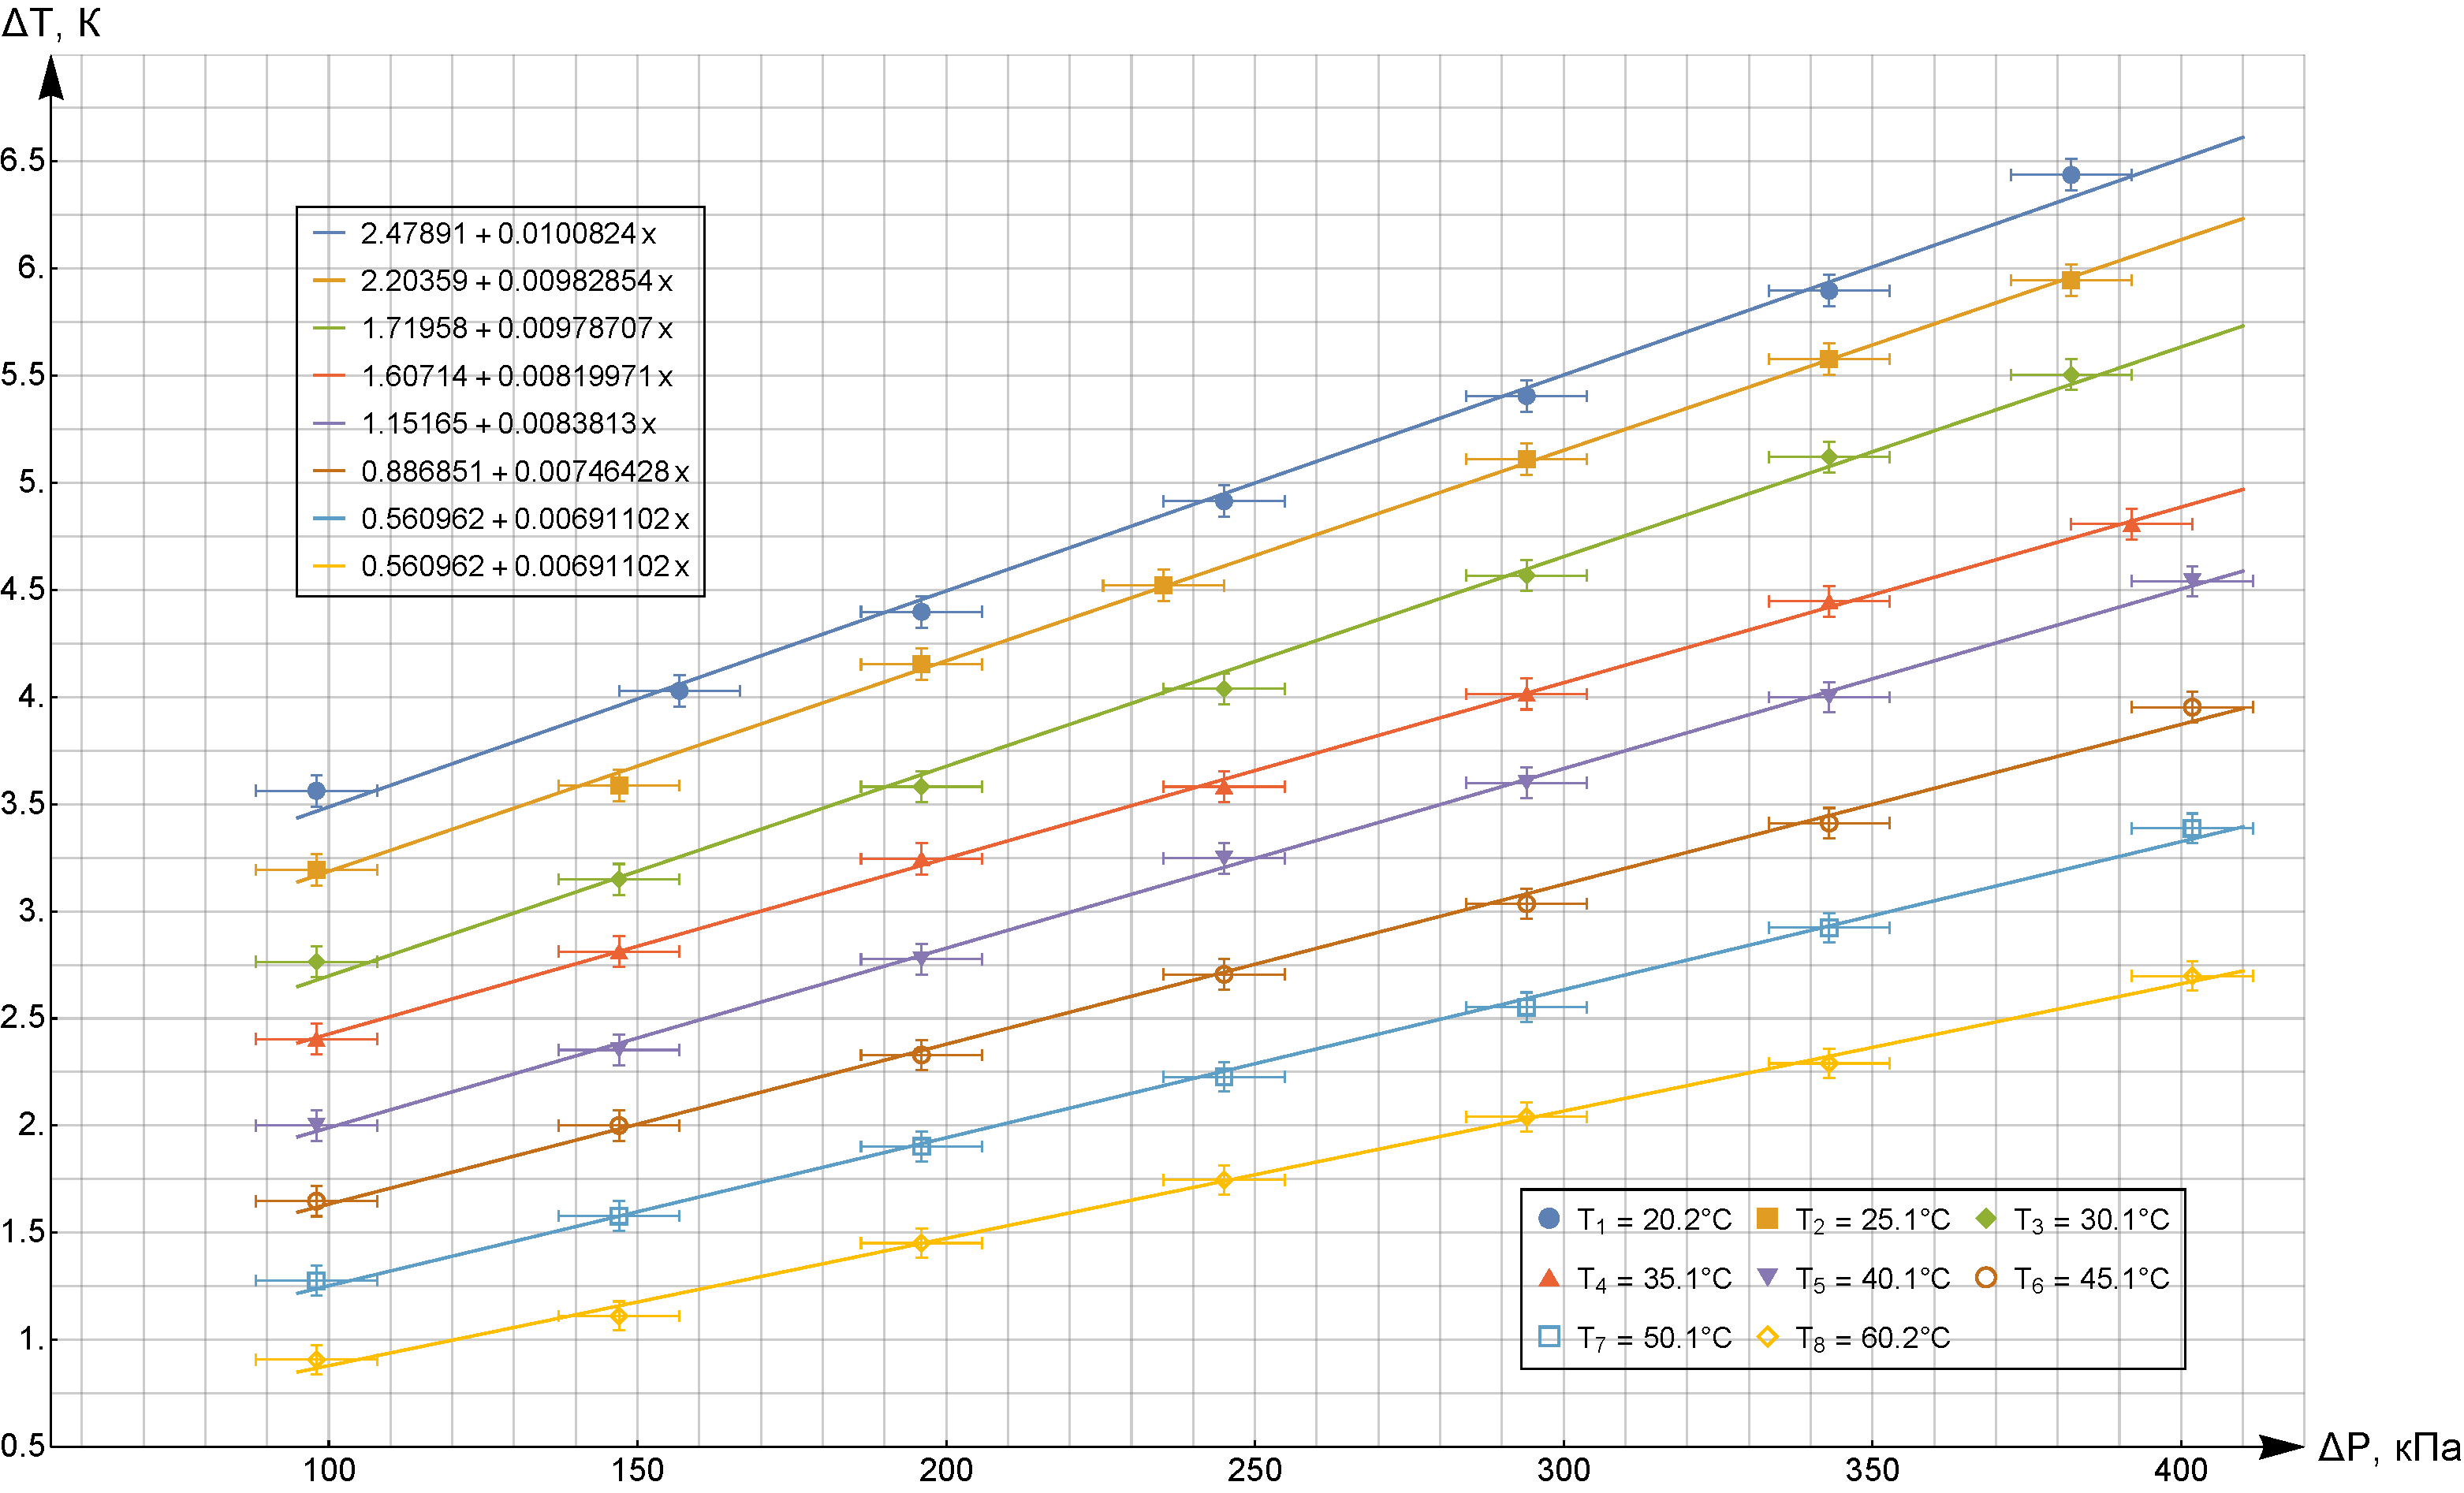
\includegraphics[width=\linewidth]{2}
		\captionsetup{justification=centering}
		\caption{График зависимости изменения температуры $\Delta T$ от изменения давления $\Delta P$ при заданной температуре $T$}
	\end{figure}

	\begin{figure}[H]
	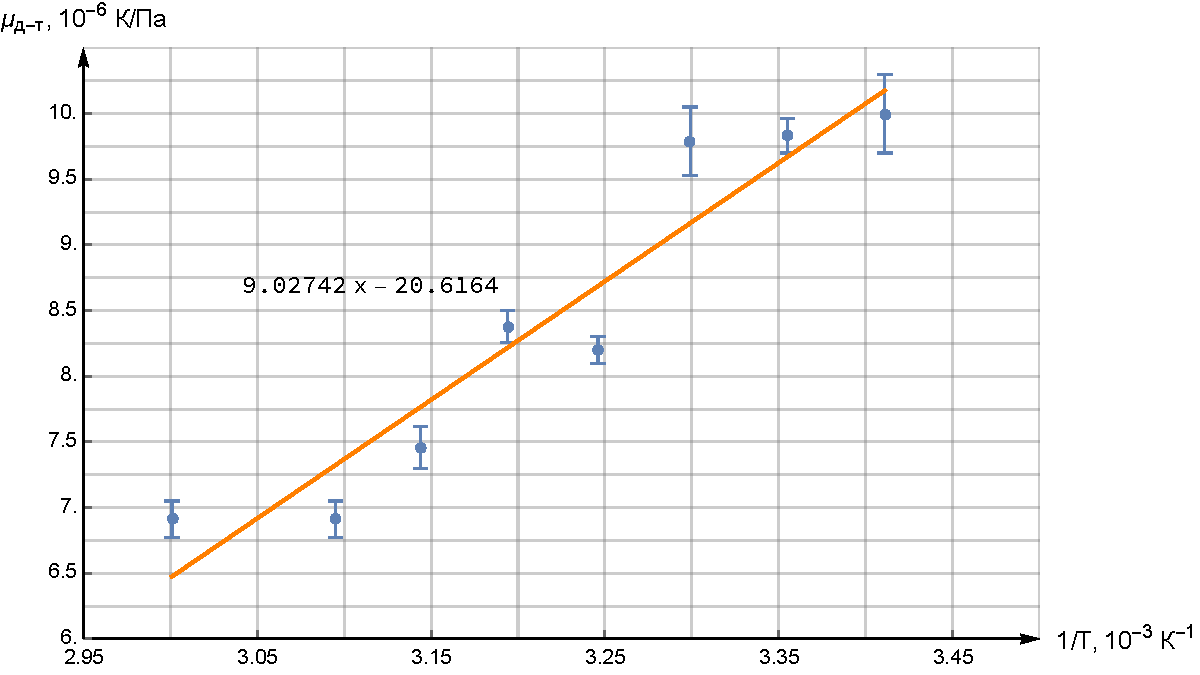
\includegraphics[width=\linewidth]{4}
	\captionsetup{justification=centering}
	\caption{График зависимости коэффициента Джоуля-Томсона $\mu_{\text{д-т}}$ от величины, обратной к температуре $1/T$}
\end{figure}
\begin{table}[H]
	\begin{center}
		\begin{tabular}{|c|c|c|c|}
			\hline
			$T,^\circ C$     & \specialcell{$1/T,$ \\$10^{-3}\cdot \text{К}^{-1} $ } & \specialcell{$\mu_{\text{д-т}},$ \\$ 10^{-6 }\cdot\text{К}/\text{Па}$}   & \specialcell{$\sigma_{\mu_{\text{д-т}}},$ \\$ 10^{-6 }\cdot\text{К}/\text{Па}$}  \\ \hline
			20,15 & 3,411 & 10,00 & 0,30  \\ \hline
			25,02 & 3,355 & 9,83  & 0,13  \\ \hline
			30,10 & 3,299 & 9,79  & 0,26  \\ \hline
			35,10 & 3,246 & 8,20  & 0,10  \\ \hline
			40,10 & 3,194 & 8,38  & 0,12  \\ \hline
			45,10 & 3,144 & 7,46  & 0,16  \\ \hline
			50,10 & 3,095 & 6,91  & 0,14  \\ \hline
			60,20 & 3,001 & 6,91  & 0,14  \\ \hline
		\end{tabular}
		\captionsetup{justification=centering}
		\caption{Зависимость коэффициента Джоуля-Томсона $\mu_{\text{д-т}}$ от величины, обратной к температуре $1/T$}
	\end{center}
\end{table}
\section{Обсуждение результатов и выводы}
В работе было определено значение дифференциального эффекта Джоуля-Томсона в зависимости от начальной температуры. Результаты в Таблице 2.

Были вычислены значения <<$a$>> и <<$b$>>  в уравнении Ван-дер-Ваальса и температура инверсии для углекислого газа.
\begin{equation*}
\begin{aligned}
	a &= (1,4\pm0,2)\  \tfrac{\text{Н}\cdot\text{м}^4}{\text{моль}^2} \\
	b& = (77\pm15)  \cdot 10^{-5} \tfrac{\text{Дж}}{\text{Па} \cdot \text{моль}}\\
	T_\text{инв}  &= (437\pm106) \ \text{К}
\end{aligned}
\end{equation*}
Значения сильно отличаются от табличных. Это может быть связано с неточностью установки и недостаточным временем ожидания установления равновесия изменения температуры при изменении давления.

Табличные значения:
\begin{equation*}
\begin{aligned}
a &= 0,365\  \tfrac{\text{Н}\cdot\text{м}^4}{\text{моль}^2} \\
b& = 42,79\  \tfrac{\text{см}^3}{\text{моль}}\\
T_\text{инв}  &= 2052 \ \text{К}
\end{aligned}
\end{equation*}

\end{document}
